\documentclass[../main.tex]{subfiles}

\begin{document}
\section{Lecture 6}{Frequency Moments and Counting Distinct Elements}

\begin{definition}
    Suppose that we receive $m$ objects (not necessarily
    distinct) that are members of the set $[n]$.
    This set of $m$ objects will, as they appear in a stream,
    be labeled $\sigma$; we have $B << m$ bits to process
    $\sigma$. Let $g$
    be a real valued non-negative function that operates on
    streams.
\end{definition}
\begin{definition}
    We say that a streaming algorithm $\mc{A}$ provides 
    $(\e, \delta)$ additive approximation if

    \[
        \prob{\abs{\mc{A} - g} > \e} < \delta
    \]
\end{definition}
J
\begin{definition}
    We say that a streaming algorithm $\mc{A}$ provides 
    $(\e, \delta)$ relative approximation if

    \[
        \prob{\frac{\mc{A}(\delta)}{g(\delta)} - 1 > \e} < \delta
    \]
\end{definition}

\begin{remark}
    Many streaming problems are trivial to solve deterministically, if we have full access to the data that enters a stream. To solve them deterministically, however, there are lower bounds on the space and running time of working algorithms. These bounds are often unacceptable. To achieve useful space and running times, thus, streaming algorithms often end up using randomized algorithms.
\end{remark}

\begin{remark}
    The task of counting how many distinct elements appear in a stream has obvious, if costly, deterministic solutions: Put all objects in a binary search tree; when a new stream object appears, search the tree for the object and, if not found, add it to the tree. We call this task the \textit{distinct elements problem}.

    This requires $O(k)$ space and $O(m \log k)$ running time where $k$ is the true number of distinct objects. Even if you were told in advance that there would be $k$ objects, a hashing solution would require $O(k)$ space and $O(m)$ running time.
\end{remark}

\begin{remark}
    A cute idea is to assume the existence of a hash function $h: [n] \rightarrow [n^3]$ that closely ``resembles'' the theoretical, non-existent hash function that maps all objects with perfect randomness to some real in $[0,1]$. Then keep track of the random varible $X = \min_{e_{i} \in \text{ all objects }} h(e_{i})$. The minimum statistic (for $k$ uniform random variables over $[0,1]$) has the property that $\Ex[X] = \frac{1}{k+1}$. Thus, at the end of streaming, take $X$, invert it and subtract $1$ from it to obtain a statistical estimator of the number of distinct objects.

    Convince yourself that the following integral represents the expectation.

    \[
        \Ex{X} = \int_{0}^{1}(\frac{1}{1-0})\binom{k}{1} (1 - x)^{k-1}
    \]

\end{remark}


\begin{theorem}
    Using the definitions set above, we can achieve a $1 + \e$ accurate estimate
    of $X$ with probability $1 - \delta$; if we kept track of the minimum hash
    value seen using only $O(\log n)$ bits, then
\end{theorem}

\subsection{BJKST}

In what follows, I give a high level overview of how to understand the analysis of BJKST

\begin{outline}
    \1 What does the algorithm do?
    \2 The algorithm repeatedly hashes elements as they appear and stores the $t$ smallest hash values.We use some hash function taken from a 2-universal hash family; moreover, this hash function has the formula $[n] \mapsto [n^3]$. It returns a statistic that depends on the average hash value of the $t$th smallest hash value.
    \1 How do we analyze the algorithm?
    \2 First, we need to understand the statistics at place. Assume that $v$ is the hash value of the $t$th smallest hash. Then:
    \3 The minimum of the hash function, assuming $d$ distinct elements would fall around $\frac{1}{d+1}$ if we were working with an ideal hash function.
    \3 Since we work over $[N]$ instead of $[0,1]^3$, however, it seems reaonable that this will instead be $\frac{N}{d+1}$. Moreover, the $t$th hash -- let's call it $v$ -- will hash to $\frac{tN}{d+1}$ on average (we're waving our hands, here). So

    \[
        v = \frac{tN}{d+1} \implies (d+1) = \frac{tN}{v} \implies \approx d = \frac{tN}{v}
    \]

    \1 We will have the algorithm described above return $\frac{tN}{v}$ as our estimate for $d$.
    We would like to have a bound of the form:

    \[
        \prob{ \abs{D - d} > \e d} \leq 1/3
    \]

    For then we can apply the median trick.
    \2 Show that there is a low chance that more than half of this experiment's trials are all bad. On average, $l/3$ of the trials will be bad; we want to bound the probability that more than $l/2$ of the trials will be bad, for that will imply the median is good.
    Use the bound $\prob{X \geq (1 + \delta)\mu} \leq \exp{\frac{-\delta^2 \mu}{3}}$.

    \1 This is decomposable into exactly two, disjoint events:

    \[
        \prob{D > d(\e+ 1)} + \prob{D < d(1 - \e)}
    \]
    \1 Focus on 
    \[
        \prob{D < d(1 - \e)}
    \]

    It is more tractable to explore this inequality when we work
    with the concrete objet $v$, the object whose hash was 
    the $t$th smallest of all hashes.
    \[
        D < d(1 - \e) \iff tN/v < d(1 - \e) \iff v > \frac{tN}{d(1 - \e)}
    \]
    \2 The foregoing occurs iff lesss than $t$ objects fell into $\frac{tN}{d(1 - \e)}$.
    \3 The probability that a single distinct element falls in this range is
    \[
        \frac{t}{d(1-\e)}
    \]
    
    Let $X = \sum_{i=1}^{d}X_{i}$. We have that

    \begin{align*}
        \Ex{X_i} &= \frac{t}{d(1 -\e)} > \frac{t(1 + \e)}{d} \\
        \Ex{X} &= \frac{t}{1 -\e} > \frac{t(1 + \e)}{1} \\
        \var{X_i} < \Ex{X_i} < \frac{t(1 + 3\e/2)}{d} \\
        \var{X} < \Ex{X} < \frac{t(1 + 3\e/2)}{1} \\
        \intertext{Notice that we were originally interested in 
            the value $\prob{X < t}$} \\
        \prob{X < t} \leq \prob{\abs{X - \Ex{X}} > \e t} \leq \var{X}/(\e t)^2 \leq \frac{t(1 + 3\e/2)}{c}\\
        \intertext{If we make $c$ sufficiently large, then we get a desireable inequality} \\
    \end{align*}

    \breathe \\
    \1 Now focus on

    \[
        \prob{D > d(\e+ 1)}
    \]
    \1 As before, we find that the event $D > d(\e + 1)$ is synonymous with the event that $v < \frac{tN}{(1 + \e)d}$.
    \2 This is the event that at least $t$ values hash inside $[1 \dots \frac{tN}{(1 + \e)d}]$
    \1 The probability that any one value hashes inside this range is
    \[
        \frac{t}{(1 + \e)d} \leq \frac{t(1 -\e/2)}{d}
    \]

    The latter inequality follows from the fact that $\frac{1}{1 + \e}$ is an alternating series\footnote{You can prove that odd partial sums are decreasing and even partial sums are increasing.} and that $\e < 1/2$.
    We want to bound

    \[
        \prob{X \geq t} 
    \]

    \begin{align*}
        \prob{X \geq t} \leq \prob{\abs{X - \Ex{X}} > \e t/2 - q} \leq \frac{4 \var{X}}{(\e t - 2q)^2} \approx \frac{4 \var{X}}{c} \\
        \intertext{Now choose $c$ to make RHS less than $\frac{1}{6}$} \\
    \end{align*}

    \2 The preceding holds, because as before, it can be shown that

    \[
        \var{X} < \frac{t(1 -\e/2)}{}
    \]

    \1 Recall that we need $c/\e^2$ elements. $c$ here is fixed, once we find a sufficiently large value for it. Thus we need $\log(1/\e^2) \log n$ bits; and we perform the median trick $\log(1 /\delta)$ times.
    \2 In total we need $O(\frac{1}{\e^2} \log(1/\delta) \log n)$ bits.
\end{outline}

\section{Lecture 7}

\begin{definition}
    A stream is a sequence $O = \left\{ e_1 \dots e_m \right\}$ where $e_i \in [n]$. For each $j \in [n]$, $f_j = \abs{O \cap j}$, which is the number of times that $j$ appears in $O$.
\end{definition}

\begin{definition}
    A function $g: \R \to \R$ of a stream $\sigma$ satisfies:

    \begin{align*}
        g(0) = 0 \\
        g(\sigma) = \sum_{i=1}^{n}g_i(f_i)
    \end{align*}
\end{definition}

\begin{example}
    Let $g_i = h(x) = x^k$ for each $i$. Then $g(\sigma)$ is the $k$th frequency moment.
\end{example}

\begin{remark}
    AMS sampling does the following:

    \begin{outline}
        \1 Draw an element $e_J$ uniformly at random from $\{e_1 \dots e_m\}$.
        \2 $e_J = i$ for some $i \in [n]$.
        \1 Count how many times $i$ appears out of $\{e_j | j \geq J\}$.
        \1 Let

        \[
            R = \abs{ \left\{ e_j | j \geq J \right\}}
        \]
        \1 Output $g_i(R) - g_i(R-1)$
    \end{outline}
\end{remark}

\begin{lemma}
    Let $Y$ be the output of AMS. Then $\Ex{Y} = g(\sigma) = \sum_{i=1}^{n}g_{i}(f_{i})$.
    \begin{center}
        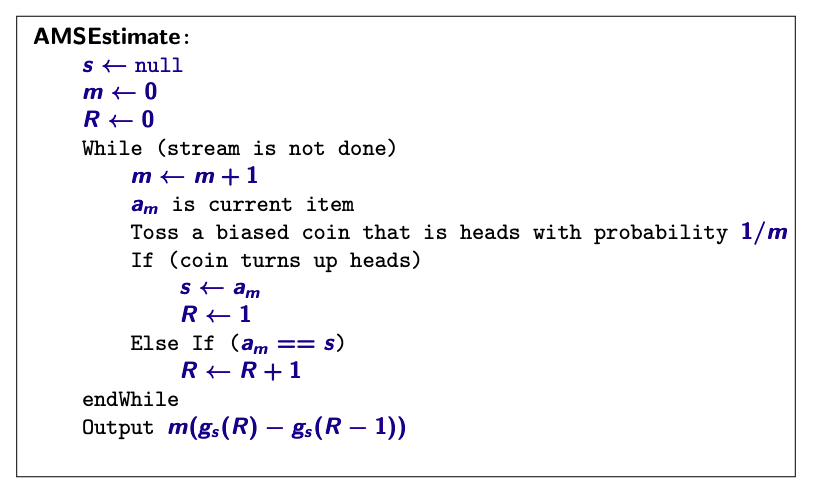
\includegraphics[width=\textwidth,height=\textheight,keepaspectratio]{lecture7_ams}
    \end{center}
\end{lemma}
\begin{proof}
    \begin{align*}
        \intertext{Let $e_J$ be the random variable whose values is the element in $[n]$ that we choose.} \\
        \Ex{Y} = \Ex{\Ex{Y | e_J}} \\
         = \sum_{i=1}^{n} \prob{e_J = i} \Ex{Y | e_J=i} \\
         = \sum_{i=1}^{n} \prob{e_J = i} \Ex{Y | e_J=i} \\
         = \sum_{i=1}^{n} \frac{f_i}{m} \Ex{Y | e_J=i} \\
         = \sum_{i=1}^{n} \frac{f_i}{m} \sum_{l=1}^{f_i}\frac{1}{f_i} m\left( g(l) = g(l-1) \right) \\
         = \sum_{i=1}^{n}g_i(f_i)
    \end{align*}
\end{proof}

\begin{remark}
    At this point, calculations are given that bound $\var{Y}$. The calculations are not very illuminating, so I omit showing them. They are at the very end of the February 5th slides:

    \url{https://courses.engr.illinois.edu/cs498abd/sp2019/slides/07.pdf}

\end{remark}


\end{document}










